\documentclass[]{article}

\usepackage{graphicx}
\usepackage{float}
\usepackage{natbib}

\renewcommand{\figurename}{Fig.}
\renewcommand{\thefigure}{S\arabic{figure}}
\renewcommand{\tablename}{Tab.}
\renewcommand{\thetable}{S\arabic{table}}

%opening
\title{Online Supplemental Material (OSM) 1: Results of Bayesian phase models for the duration of pottery styles in the Congo Basin}
\author{Dirk Seidensticker}

\begin{document}

\maketitle

\begin{figure}[H]
	\centering
	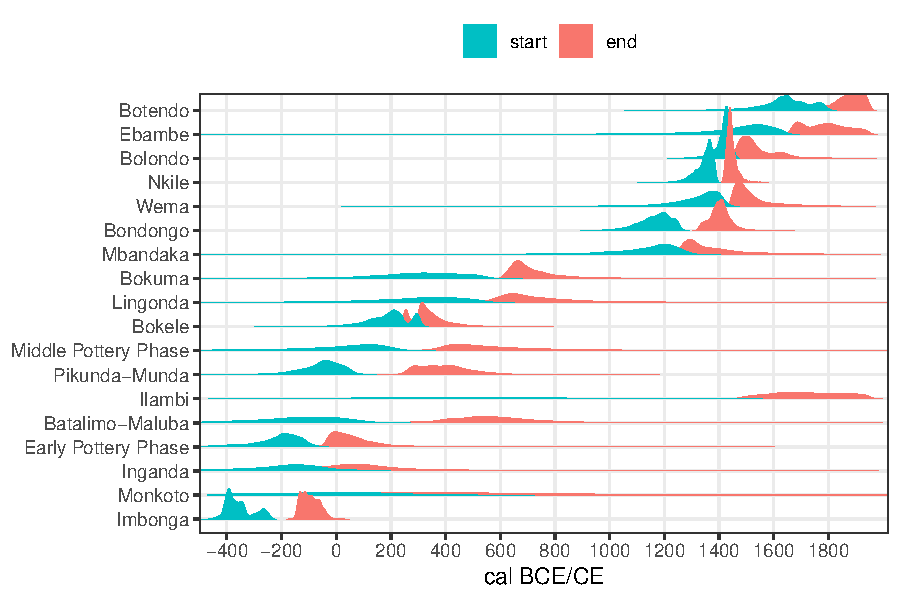
\includegraphics[width=\textwidth]{fig_bayesphases.pdf}
	\caption{Alpha distributions of Bayesian phase models for the duration of pottery styles \citep[cf.][]{Crema.2020a,Crema.2021a} that are dated via at least two reliable radiocarbon dates.}
	\label{fig:bayes}
\end{figure}

\begin{table}[H]
	\centering
	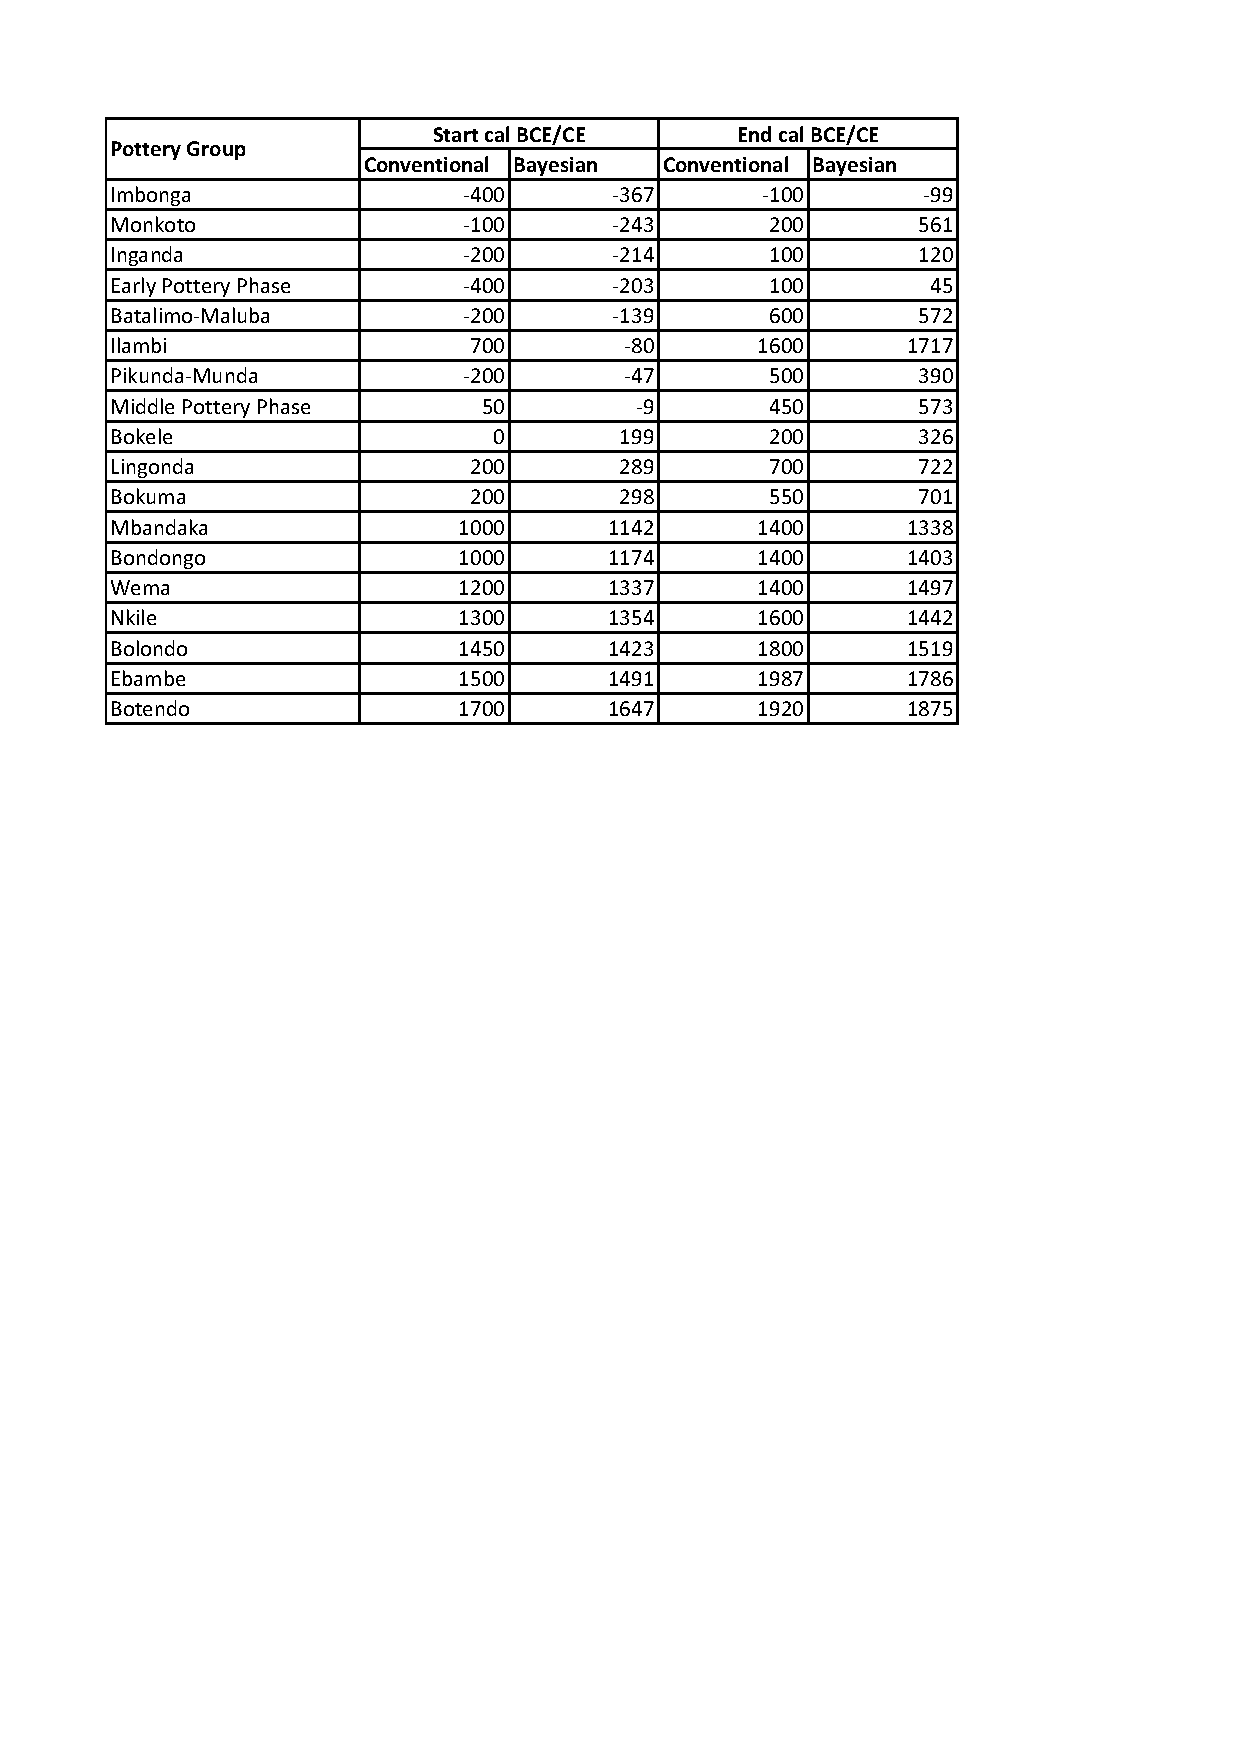
\includegraphics[width=\textwidth]{tbl_bayesphases_comparison.pdf}
	\caption{Comparison between conventional start and end dates for radiocarbon dated pottery groups in the Congo Basin \citep[Data S2]{Seidensticker.2021} and median start and end calendar years derived from Bayesian phase determination (Fig.~\ref{fig:bayes}).}
	\label{tab:bayes}
\end{table}

\begin{figure}[H]
	\centering
	\includegraphics[width=\textwidth]{fig_s_map_time_slices_congobasin_total.pdf}
	\caption{Time-sliced maps of occurrences of pottery styles in the Congo Basin. If multiple contemporaneous pottery styles were recorded at a site, the colored icon is divided following \citet[218--244 Fig.~100--107]{Seidensticker.2021e}. The extent of the map is equal to Fig. 1 and colors correspond to Fig. 2.}
	\label{fig:timeslices_overview}
\end{figure}

\bibliographystyle{spbasic}
\bibliography{references.bib}

\end{document}
